%==============================================================================%
% Documentation for NSTexam.cls (LaTeX package for NST papers).                %
%                                                                              %
% D. A. Green --- MRAO --- 2014 October (for Version 7.4).                       %
%==============================================================================%
\documentclass[txfonts]{NSTexam}
%\documentclass[newtx]{NSTexam}
\listfiles
%
\usepackage{graphicx}
\usepackage{amsmath} % For \tag
\usepackage{pgfplots}



\usepackage{tikz}
\usetikzlibrary{trees}
\usetikzlibrary{decorations.pathmorphing}
\usetikzlibrary{decorations.markings}


  \definecolor{jblue}  {RGB}{20,50,100}
  \definecolor{lblue}  {RGB}{40,100,240}
  \definecolor{npurple}  {RGB} {153, 51, 204}
  \definecolor{wred}   {RGB}{217,0,56}
  \definecolor{white}   {RGB}{255,255,255}
  
  \definecolor{korange}   {RGB}{235, 80,  43}
  \definecolor{korange2}   {RGB}{245, 100,  63}
  \definecolor{kyelloworange}   {RGB}{255, 210,  110}
  \definecolor{kyelloworange2}   {RGB}{240, 170,  90}
  \definecolor{kred}   {RGB}{204,  102, 153}
  \definecolor{kpurple}   {RGB}{153,  61, 190}
  \definecolor{kpurplelight}   {RGB}{213,  161, 230}

          % Define styles for the different kind of edges in a Feynman diagram
  \tikzset{
    photon/.style={decorate, decoration={snake}, draw=npurple,very thick},
    boson/.style={decorate, decoration={snake}, draw=npurple,very thick},
    electron/.style={draw=jblue,very thick, postaction={decorate},
             decoration={markings,mark=at position .55 with {\arrow[draw=jblue]{>}}}
    },
    electron2/.style={draw=jblue,very thick, postaction={decorate},
             decoration={markings,mark=at position .55 with {\arrow[draw=jblue]{<}}}
    },
    fermion/.style={draw=jblue,very thick, postaction={decorate},
              decoration={markings,mark=at position .55 with {\arrow[draw=jblue]{}}}
    },
    gluon/.style={decorate, draw=korange,very thick, %kred
      decoration={coil,amplitude=4pt, segment length=6pt}},
    higgs/.style={draw=wred,very thick, postaction={decorate},
             decoration={markings,mark=at position .55 with {\arrow[draw=wred]{>}}}
    },
    nothing/.style={draw=white,very thick}
  }





%
\nofiles
%
%\showanswerstrue
%
\begin{document}
%------------------------------------------------------------------------------%
\ID{A}
\version{V7.4}

\tripos{NATURAL SCIENCES TRIPOS: Part III Physics}
\tripos{MASTER OF ADVANCED STUDY IN PHYSICS}
\tripos{NATURAL SCIENCES TRIPOS: Part III Astrophysics}
\date{Tuesday 17 January 2017:      14:00 to 16:00}
\paper{MAJOR TOPICS}
\paper{Paper 1/PP (Particle Physics)}

\begin{rubric}
%
Answer {\textbf{two}} questions only.  The approximate number of marks allocated to each part of a question is indicated in the right-hand margin where appropriate. The paper contains four sides including this one and is accompanied by a book giving values of constants and containing mathematical formulae which you may quote without proof.

You should use a {\textbf{separate Answer Book}} for each question.
%
\end{rubric}

\requirements{
              2x20-page answer books\\Rough workpad}{Mathematical Formulae Handbook\\
                             Approved calculator allowed}

\warning

\newpage
%------------------------------------------------------------------------------%
\sectionfalse


\begin{questions} 

\newcommand{\bookwork}[1]{{\bf BOOKWORK[ #1 ] }}
\newcommand{\fourvec}[4]{\left(\begin{array}{c}#1\\#2\\#3\\#4\end{array}\right)}
 \newcommand*\circled[1]{\tikz[baseline=(char.base)]{
     \node[shape=circle,draw,inner sep=2pt] (char) {#1};}}
                        
                        
\question 


\newcommand\diaguchannel{{ 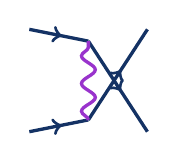
\begin{tikzpicture}[scale=0.5,
                     thick,
             % Set the overall layout of the tree
             level/.style={level distance=3.15cm, line width=0.4mm},
             leve/l 2/.style={sibling angle=60},
             leggvel 3/.style={sibling angle=60},
             level 4/.style={level distance=1.4cm, sibling angle=60}
     ]
 %Incoming p1
     \draw[jblue,very thick,electron] (-1.5,1.3) -- (0,1) ;
 %Outgoing p3
     \draw[jblue,very thick,electron] (0,-1) -- (1.5,1.3) ;
 %Incoming p2
     \draw[jblue,very thick,electron] (-1.5,-1.3) -- (0,-1) ;
 %Outgoing p4
     \draw[jblue,very thick,electron] (0,+1) -- (1.5,-1.3) ;
 % photon
     \draw[jblue,very thick,photon] (0,-1) -- (0,1) ;
 %% arrow
 %    \draw[jblue,very thick,->] (-3.30,-0.5) -- (-3.00,-0.95) ;
 \end{tikzpicture}
}}

\newcommand\diagtchannel{{ 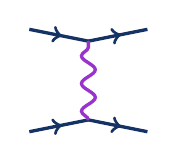
\begin{tikzpicture}[scale=0.5,
                     thick,
             % Set the overall layout of the tree
             level/.style={level distance=3.15cm, line width=0.4mm},
             level 2/.style={sibling angle=60},
             level 3/.style={sibling angle=60},
             level 4/.style={level distance=1.4cm, sibling angle=60}
     ]
 %Incoming p1
     \draw[jblue,very thick,electron] (-1.5,1.3) -- (0,1) ;
 %Outgoing p3
     \draw[jblue,very thick,electron] (0,1) -- (1.5,1.3) ;
 %Incoming p2
     \draw[jblue,very thick,electron] (-1.5,-1.3) -- (0,-1) ;
 %Outgoing p4
     \draw[jblue,very thick,electron] (0,-1) -- (1.5,-1.3) ;
 % photon
     \draw[jblue,very thick,photon] (0,-1) -- (0,1) ;
 %% arrow
 %    \draw[jblue,very thick,->] (-3.30,-0.5) -- (-3.00,-0.95) ;
 \end{tikzpicture}
}}

\newcommand\diagtchannelback{{ 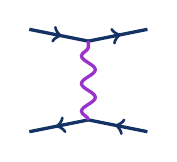
\begin{tikzpicture}[scale=0.5,
                     thick,
             % Set the overall layout of the tree
             level/.style={level distance=3.15cm, line width=0.4mm},
             level 2/.style={sibling angle=60},
             level 3/.style={sibling angle=60},
             level 4/.style={level distance=1.4cm, sibling angle=60}
     ]
 %Incoming p1
     \draw[jblue,very thick,electron] (-1.5,1.3) -- (0,1) ;
 %Outgoing p3
     \draw[jblue,very thick,electron] (0,1) -- (1.5,1.3) ;
 %Incoming p2
     \draw[jblue,very thick,electron] (0,-1) -- (-1.5,-1.3) ;
 %Outgoing p4
     \draw[jblue,very thick,electron] (1.5,-1.3) -- (0,-1);
 % photon
     \draw[jblue,very thick,photon] (0,-1) -- (0,1) ;
 %% arrow
 %    \draw[jblue,very thick,->] (-3.30,-0.5) -- (-3.00,-0.95) ;
 \end{tikzpicture}
}}

\newcommand\diagschannel{{ 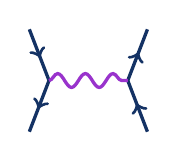
\begin{tikzpicture}[scale=0.5,
                      thick,
              % Set the overall layout of the tree
              level/.style={level distance=3.15cm, line width=0.4mm},
              level 2/.style={sibling angle=60},
              level 3/.style={sibling angle=60},
              level 4/.style={level distance=1.4cm, sibling angle=60}
      ]
  %Incoming p1
      \draw[jblue,very thick,electron] (-1.5,1.3) -- (-1,0) ;
  %Incoming p2
      \draw[jblue,very thick,electron] (-1,0) -- (-1.5,-1.3) ;
  %Outgoing p3
      \draw[jblue,very thick,electron] (1,0) -- (1.5,1.3) ;
  %Outgoing p4
      \draw[jblue,very thick,electron] (1.5,-1.3) -- (1,0) ;
  % photon
      \draw[jblue,very thick,photon] (-1,0) -- (1,0) ;
  %% arrow
  %    \draw[jblue,very thick,->] (-3.30,-0.5) -- (-3.00,-0.95) ;
  \end{tikzpicture}
 }}


\newcommand\diagemuSS{\diagtchannel}
\newcommand\diagannihil{\diagschannel}
\newcommand\diagTU    {\diagtchannel-\diaguchannel}
\newcommand\diagTS    {\diagtchannelback + \diagschannel}
\newcommand\diagemuOS {\diagtchannelback}
\newcommand\diagbadone{no tree level diagram}
\newcommand\diagbadtwo{no tree level diagram}
\newcommand\diageRmuR {\diagtchannel}
\newcommand\diageRmuL {\diagtchannel}
\newcommand\diagbadthr{no tree level diagram}




\newcommand\procgeneric{{$a b           \rightarrow c d        $}}
\newcommand\procemuSS  {{$e^- \mu^-     \rightarrow e^-   \mu^-$}}
\newcommand\procannihil{{$e^- e^+       \rightarrow \mu^- \mu^+$}}
\newcommand\procmoeller{{$e^- e^-       \rightarrow e^-   e^-  $}}
\newcommand\procbhabha {{$e^- e^+       \rightarrow e^-   e^+  $}}
\newcommand\procemuOS  {{$e^- \mu^+     \rightarrow e^-   \mu^+$}}
\newcommand\procbadone {{$e^- \mu^+     \rightarrow e^+   \mu^-$}}
\newcommand\procbadtwo {{$e^- e^-       \rightarrow \mu^- \mu^-$}}
\newcommand\procbadthr {{$e^-_R e^+_R   \rightarrow \mu^- \mu^+$}}
\newcommand\proceRmuR  {{$e^-_R \mu^-_R \rightarrow e^-   \mu^-$}}
\newcommand\proceRmuL  {{$e^-_R \mu^-_L \rightarrow e^-   \mu^-$}}

\newcommand\numberemuSS  {\circled{0}}
\newcommand\numberannihil{\circled{1}}
\newcommand\numbermoeller{\circled{2}}
\newcommand\numberbhabha {\circled{3}}
\newcommand\numberemuOS  {\circled{4}}
\newcommand\numberbadone {\circled{5}}
\newcommand\numberbadtwo {\circled{6}}
\newcommand\numbereRmuR  {\circled{7}}
\newcommand\numbereRmuL  {\circled{8}}
\newcommand\numberbadthr {\circled{9}}

% axis style
\pgfplotsset{every axis/.append style={
                    axis x line=bottom,    % put the x axis in the middle
                    axis y line=middle,    % put the y axis in the middle
                    %axis line style={<->}, % arrows on the axis
                    %xlabel={$\cos\theta$},          % default put x on x-axis
                    %ylabel={$\frac{d\sigma_{\text{numerator}}}{d\cos\theta}$},          % default put y on y-axis
                    xtick=\empty,
                    %xtick={-1,0,+1},
                    ytick=\empty,
    %                ylabel style={at=(current axis.above origin), anchor=south},
    %xmin=-1,xmax=1, 
    ymin=0, ymax=2, minor y tick num=2
                    }}

% line style
\pgfplotsset{mystyle/.style={color=blue,no marks,line width=1pt}} 

\pgfplotsset{width=3cm} 

% arrow style: stealth stands for 'stealth fighter' 
%\tikzset{>=stealth}

\newcommand\myplot[1]{{\begin{tikzpicture}
    \begin{axis}[
        %ylabel={$f(\cos\theta)$},          % default put y on y-axis
                    xmin=-1,xmax=1
    ]
            %xmin=-1,xmax=1, ymin=0, ymax=2, minor y tick num=2
        \addplot[mystyle] expression[domain=-1:1,samples=100]{#1} ;
    \end{axis}
\end{tikzpicture}
}}
\newcommand\myploot[1]{{\begin{tikzpicture}
    \begin{axis}[
        %ylabel={$\text{ans}(\cos\theta)$},          % default put y on y-axis
                    xmin=-0.99,xmax=0.99%,ymax=4
                ]
            %xmin=-1,xmax=1, ymin=0, ymax=2, minor y tick num=2
        \addplot[mystyle] expression[domain=-0.95:0.95,samples=100]{#1} ;
    \end{axis}
\end{tikzpicture}
}}

\newcommand\msqemuSS  {{$\frac{s^2+u^2}{t^2}$}}
\newcommand\msqannihil{{$\frac{t^2+u^2}{s^2}$}}
\newcommand\msqmoeller{{$\frac{s^2+u^2}{t^2}+\frac{2 s^2}{tu}+\frac{s^2+t^2}{u^2}$}}
\newcommand\msqbhabha {{$\frac{s^2+u^2}{t^2}+\frac{2 u^2}{ts}+\frac{t^2+u^2}{s^2}$}}
\newcommand\msqemuOS  {{\msqemuSS
%\ probably
}}
\newcommand\msqbadone {{$0$}}
\newcommand\msqbadtwo {{$0$}}
\newcommand\msqbadthr {{$0$}}
\newcommand\msqeRmuR  {{$\frac{s^2}{t^2}$}}
\newcommand\msqeRmuL  {{$\frac{u^2}{t^2}$}}


\newcommand\plothighdip{{\myplot{0.25*(1-x)*(1-x)+0.25*(1+x)*(1+x)}}}
\newcommand\plotflat{{\myplot{1}}}
\newcommand\plotBWDbias{{\myplot{0.5*(1-x)*(1-x)}}}
\newcommand\plotFWDbias{{\myplot{0.5*(1+x)*(1+x)}}}
%\newcommand\plotzero{{\myplot{0}}}
\newcommand\plotzero{}
\newcommand\plotfwdbias{{\myplot{1+0.25*(1+x)*(1+x)}}}
\newcommand\plotbwdbias{{\myplot{1+0.25*(1-x)*(1-x)}}}


\newcommand\ploothighdip{{\myploot{0.25*(1-x)*(1-x)+0.25*(1+x)*(1+x)}}}
\newcommand\plootflat{{\myploot{1/((1-x)*(1-x))}}}
\newcommand\plootBWDbias{{\myploot{0.5*(1-x)*(1-x)/((1-x)*(1-x))}}}
\newcommand\plootFWDbias{{\myploot{0.5*(1+x)*(1+x)/((1-x)*(1-x))}}}
%\newcommand\plootzero{{\myploot{0}}}
\newcommand\plootzero{}
\newcommand\plootfwdbias{{\myploot{(1+0.25*(1+x)*(1+x))/((1-x)*(1-x))}}}
\newcommand\plootbwdbias{{\myploot{(1+0.25*(1-x)*(1-x))/((1-x)*(1-x))}}}

\newcommand\plootTU{{\myploot{(
            (1+0.25*(1+x)*(1+x))/((1-x)*(1-x)) 
+
            8/((1-x)*(1+x)) 
+
            (1+0.25*(1-x)*(1-x))/((1+x)*(1+x)) 
            )/32
}}}
\newcommand\plootTS{{\myploot{(
            (1+0.25*(1+x)*(1+x))/((1-x)*(1-x)) 
+
2*0.25*(1+x)*(1+x)/(-0.5*(1-x)    * 1) 
+
(0.25*(1-x)*(1-x)+0.25*(1-x)*(1-x))/(1) 
            )/4
}}}

\newcommand\plotannihil{{\plothighdip}}
\newcommand\plotemuSS{{\plotfwdbias}}
\newcommand\plotemuOS{{\plotfwdbias}}
\newcommand\plotbadone{{\plotzero}}
\newcommand\plotbadtwo{{\plotzero}}
\newcommand\plotbadthr{{\plotzero}}
\newcommand\ploteRmuR{{\plotflat}}
\newcommand\ploteRmuL{{\plotFWDbias}}

\newcommand\plootannihil{{\ploothighdip}}
\newcommand\plootemuSS{{\plootfwdbias}}
\newcommand\plootemuOS{{\plootfwdbias}}
\newcommand\plootbadone{{\plootzero}}
\newcommand\plootbadtwo{{\plootzero}}
\newcommand\plootbadthr{{\plootzero}}
\newcommand\plooteRmuR{{\plootflat}}
\newcommand\plooteRmuL{{\plootFWDbias}}

\newcommand\labeRmuL{\circled{A}}
\newcommand\labmoeller{\circled{B}}
\newcommand\labannihil{\circled{C}}
\newcommand\labemuSS{\circled{D}}
\newcommand\labemuOS{\circled{D}}
\newcommand\labeRmuR{\circled{E}}
\newcommand\labbhabha{\circled{F}}
\newcommand\notallowed{{$\begin{array}{c}\text{not}\\ \text{allowed}\end{array}$}}
\newcommand\labbadone{\notallowed}
\newcommand\labbadtwo{\notallowed}
\newcommand\labbadthr{\notallowed}


\newcounter{lestercounter}
%
%
%\begin{parts}
%
%
%\part
%\end{parts}
%
%\setcounter{lestercounter}{\value{partcount}}
%
%\noindent The `Bjorken $x$' observable is {\em defined} by the equation $x=-{q^2} /{(2 p_2 . q)}$.  If $x$ is re-expressed in terms of the independent variables contained within $S$ in the Zarquon model, `Bjorken $x$' may be shown to be equal to
%\begin{align}\frac{\sqrt{m^2+a^2}+a\cos\alpha}{M}\left({1-\frac{a \rho}{p} }\right)^{-1}\tag{$\star$}\end{align}where $\rho=\cot{\frac\theta 2} \sin\alpha \sin\delta + \cos\alpha$.  \shorthint{You are not asked to show this!}


%\myplot{x*x}
%\myplot{1-x*x}

The Mandelstam variables $s$, $t$ and $u$ for $2\rightarrow 2$ scattering processes are defined as
$s=(p_1+p_2)^2$, $t=(p_1-p_3)^2$ and $u=(p_1-p_4)^2$, where $p_1$ and $p_2$ are incoming four-momenta and $p_3$ and $p_4$ are outgoing four-momenta.  Within this question you may neglect the masses of all incoming and outgoing particles.
\begin{parts}
    \part
    Show that $s$, $t$ and $u$ are not independent by considering $s+t+u$. \marks{2}
    \answer

    \bookwork{One of the example sheet questions required students to show that $$s+t+u=m_1^2+m_2^2+m_3^2+m_4^2,$$ which is a statement that was also made in Lecture 1 and printed on Handout 1, so this question (which asks for less since all masses may be neglected) is bookwork.  One mark for simply stating that $s+t+u=0$ (even if given without proof) and another for giving some clear indication that it follows from momentum conservation .... perhaps by writing $$s+t+u=2 p_1.p_2 -2 p_1.p_3 - 2 p_1.p_4 = 2 p_1.(p_2-p_3-p_4) = 2
    p_1.(-p_1)=-2m_1^2 =0.$$}
    \endanswer
    \part
    Find $s$, $t$ and $u$ in terms of $p$ and $\theta$, where $p$ is the magnitude of the three-momentum of $p_1$ in the centre-of-mass frame, and $\theta$ is the angle between the spatial parts of $p_1$ and $p_3$ in that same frame.\marks{4}
\setcounter{lestercounter}{\value{partcount}}
    \answer

    \bookwork{
        \begin{align}
            s=((p,0,0,p)+(p,0,0,-p))^2=4p^2 \qquad\text{(one mark)}
        \end{align}
      \begin{align}
          t &=((p,0,0,p)-(p,p\sin\theta,0,p\cos\theta))^2\\
            &= (0,-p\sin\theta,0,p(1-\cos\theta))^2 \\
            &= -p^2\sin^2\theta-p^2(1-\cos\theta)^2 \\
            &= p^2(-\sin^2\theta -1-\cos^2\theta)+2p^2\cos\theta \\
            &= -2 p^2(1-\cos\theta ) \qquad\text{(two marks)}
      \end{align}
      \begin{align}
          u &=((p,0,0,p)-(p,-p\sin\theta,0,-p\cos\theta))^2\\
            &= (0,p\sin\theta,0,p(1+\cos\theta))^2 \\
            &= -p^2\sin^2\theta-p^2(1+\cos\theta)^2 \\
            &= p^2(-\sin^2\theta -1 -cos^2\theta)-2p^2\cos\theta \\
            &= -2 p^2(\cos\theta +1) \qquad\text{(two marks).}
      \end{align}
      Note this means that $t^2=\frac 1 4 (1-\cos\theta)^2 s^2$ and $u^2=\frac 1 4 (1+\cos\theta)^2 s^2$.
    }
    \endanswer
\end{parts}
Ten scattering processes (numbered $\circled{0}$ to $\circled{9}$) and six quantities (denoted $\circled{A}$ to $\circled{F}$) are listed in the following tables.
\vspace{0.5cm}

\begin{tabular}{|cc|cc|}
%                   & \procgeneric  & \msqemuSS   \\
    \hline
    \numberemuSS   & \procemuSS    & 
    \numberbadone  & \procbadone   \\ \hline
    \numberannihil & \procannihil  & 
    \numberbadtwo  & \procbadtwo   \\ \hline
    \numbermoeller & \procmoeller  & 
    \numbereRmuR   & \proceRmuR    \\ \hline
    \numberbhabha  & \procbhabha   & 
    \numbereRmuL   & \proceRmuL    \\ \hline
    \numberemuOS   & \procemuOS    & 
    \numberbadthr  & \procbadthr   \\ \hline
\end{tabular}\qquad
\begin{tabular}{|cc|}
%                   & \procgeneric  & \msqemuSS   \\
    \hline
   \labeRmuL     & \msqeRmuL     \\ \hline
   \labmoeller   & \msqmoeller   \\ \hline
   \labannihil   & \msqannihil   \\ \hline
   \labemuSS     & \msqemuSS     \\ \hline
   \labeRmuR     & \msqeRmuR     \\ \hline
   \labbhabha    & \msqbhabha    \\ \hline
%   \circled{G}   & `other' (see text)        \\ \hline
\end{tabular}
\vspace{0.5cm}

\noindent Each of the quantities $\circled{A}$ to $\circled{F}$ represents the square of the modulus of the tree-level QED spin-averaged matrix element $\left<|M|^2\right>$ of one or more of the processes $\circled{0}$ to $\circled{9}$, after omission of any overall factors that do not depend on $s$, $t$ or $u$. For each process the particle names are given in the order corresponding to momentum labels $p_1 p_2 \rightarrow p_3 p_4$.
\begin{parts}
 \setcounter{partcount}{\value{lestercounter}}
    \part
    Determine which (if any) of the processes in $\circled{0}$ to $\circled{9}$ are `allowed' at tree-level in QED, and which (if any) are correspondingly `not allowed'.\marks{1}
    \part 
    For each `allowed' process in $\circled{0}$ to $\circled{9}$, in turn:
    \begin{subparts}
        \subpart
        draw all the tree-level QED Feynman diagrams for that process;
    \subpart
   identify the quantity in $\circled{A}$ to $\circled{F}$ which represents the $s$, $t$ and $u$ dependence of $\left< |M|^2\right>$ for that process, explaining your reasoning; and  
   %If you believe there are any cases where the required dependence is not found in $\circled{A}$ to $\circled{F}$ then select $\circled{G}$ (`other') and describe in your own words the nature of the dependence on $s$, $t$ and/or $u$.
   \subpart
   qualitatively sketch the $\cos\theta$ dependence of $\left< |M|^2\right>$.
\end{subparts}
\marks{23}
\shorthint{Hint: Answers to part (ii) need not contain lengthy mathematical proofs or deriavations from first-principles where simpler arguments can be found.   }
\end{parts}

\answer


%$$
%s=(p_1+p_2)^2=(2p,0,0,0)^2=4 p^2
%$$
%
%$$
%t=(p_1-p_3)^2=(0,-p\sin \theta,0,p-p\cos\theta)^2=-p^2 \sin^2\theta-p^2(1-cos\theta)^2=-2 p^2 (1-\cos\theta)
%$$
%
%$$
%u=(p_1-p_4)^2=(0,p\sin \theta,0,p+p\cos\theta)^2=p^2 \sin^2\theta-p^2(1+cos\theta)^2=2 p^2 (1+\cos\theta)
%$$

The main parts of the answer are as summarised in the following table:

\noindent \begin{tabular}{|c|c|c|c|c|c|c|}
%                   & \procgeneric  & \msqemuSS   \\
    \hline 
    & process &  & $\propto \left< {{\left|{M}\right|}^2} \right> $ & numerator & whole & diagram \\
    & &  & & sketch & sketch & \\
    & &  & & (info only) & $[-1,1]$ & \\
    \hline
    \numberemuSS   & \procemuSS    & \labemuSS   & \msqemuSS   & \plotemuSS   & \plootemuSS   & \diagemuSS   \\ \hline
    \numberannihil & \procannihil  & \labannihil & \msqannihil & \plotannihil & \plootannihil & \diagannihil \\ \hline
    \numbermoeller & \procmoeller  & \labmoeller & \msqmoeller &              & \plootTU      & \diagTU      \\ \hline
    \numberbhabha  & \procbhabha   & \labbhabha  & \msqbhabha  &              & \plootTS      & \diagTS      \\ \hline
    \numberemuOS   & \procemuOS    & \labemuOS   & \msqemuOS   & \plotemuOS   & \plootemuOS   & \diagemuOS   \\ \hline
    \numberbadone  & \procbadone   & \labbadone  & \msqbadone  & \plotbadone  & \plootbadone  & \diagbadone  \\ \hline
    \numberbadtwo  & \procbadtwo   & \labbadtwo  & \msqbadtwo  & \plotbadtwo  & \plootbadtwo  & \diagbadtwo  \\ \hline
    \numbereRmuR   & \proceRmuR    & \labeRmuR   & \msqeRmuR   & \ploteRmuR   & \plooteRmuR   & \diageRmuR   \\ \hline
    \numbereRmuL   & \proceRmuL    & \labeRmuL   & \msqeRmuL   & \ploteRmuL   & \plooteRmuL   & \diageRmuL   \\ \hline
    \numberbadthr  & \procbadthr   & \labbadthr  & \msqbadthr  & \plotbadthr  & \plootbadthr  & \diagbadthr  \\ \hline
\end{tabular}
The last two non-zero Feynman diagrams implicitly contain only one spin combination each ($RR\rightarrow RR$ and $RL\rightarrow RL$ respectively) while all others non-zero diagrams implicity average over four incoming spin combinations, in terms of which the outgoing spins are fixed by the rule that the helicity arrows (not drawn) pass through each QED vertex without changing direcection (i.e. one helicity arrow into and one out of each vertex, or vice versa).  The assignments of quantity labels to process labels may be done as follows:
\begin{enumerate}
\item
The three `impossible' processes can be immediately identified by either the lack of a valid lepton flavour conserving Feynman diagram  (\numberbadone:\procbadone\ and \numberbadtwo:\procbadtwo) or lack of helicity conservation (\numberbadthr:\procbadthr). These are all therefore \labbadone\ with a zero matrix element having no releveant dependence on $s$, $t$ or $u$.
\item
There is only one $s$-channel Feynman diagram (\diagannihil\ for \numberannihil:\procannihil), and only one quantity in the list having an $s^2$ in the denominator (\labannihil:\msqannihil).  The wording of the question informs us that every listed quantity corresponds to at least one of the listed processes, so these two must be one and the same. Furthermore, most students should recall that this is the first diagram they computed in lectures.  They saw computed the angular dependence of the numerator (proportional to $(1+\cos\theta)^2 + (1-\cos\theta)^2$) not only using spinors and a sum of modulus squares of Lorentz dot products of electron and muon currents, but also by considering the angular dependence of the initial state.  In the case of the latter, it was noted that thie initial state was either $\left|1,+1\right>$ or $\left|1, -1\right>$ and so either full backward (or respectively full forward) scattering of the electron would be impossible and indicated a $(1\pm\cos\theta)^2$ dependence in the numerator. These recollections can be compared to th values for $t$ and $u$ just found in the earlier part of this question, to reconfirm that the numerator supplied agrees with those facts.
\item
There are four pure $t$-channel Feynam diagrams (\numberemuOS:\procemuOS, \numberemuSS:\procemuSS, \numbereRmuR:\proceRmuR\ and \numbereRmuL:\proceRmuL) and three pure $t$-channel quantities (\labemuOS:\msqemuOS, \labeRmuR:\msqeRmuR\ and \labeRmuL:\msqeRmuL). Given that every listed quantity corresponds to at least one of the listed processes, this means that 
%either: each one of these quantities is used once with one process while a single `other' (\labbadone) is needed for the remaining process, or 
two of these quantities are used once and the other is used twice. On close inspection it should become readily apparent that the two processes with specified initial spins (\numbereRmuR:\proceRmuR\ and \numbereRmuL:\proceRmuL) are just two of the four fixed-helicity initial states that need to be considered when looking at \numberemuSS:\procemuSS.  The first is a mixture of $\left|1,0\right>$ and $\left|0,0\right>$ without any preferred $z$-component of spin, and so must have an isotropic numerator of
which $s^2$ is the only possiblity.  The second is a $\left|1,1\right>$ state which (by helicity conservation in each vertex will prefer to forward scatter (and cannot fully backward scatter), as discussed in the lectures, and so must have a $(1+\cos\theta)^2$ numerator which we have already seen is proportional to $t^2$.  The same would be true for the other two of the four fixed-helicity states not considered.  Therefore it can be seen that \msqeRmuR\ is \proceRmuR, \msqeRmuL\ is \proceRmuL,
and their sum \msqemuSS\ must be \procemuSS.  This leaves \procemuOS.  %Does it need a \labbadone?  No it does not. 
After a little thought it shoud be apparent that the only difference between it and \procemuSS\ is the sign of the muon.  This might matter if we were looking at the Weak interaction which threats the L and R parts of particles and antiparticles differently, but the students have seen in this course that the QED vertex does not treat particles and anti-particles differently. It
is true that the muon to anti-muon change will generate a sign change in the matrix element, but this will disappear when it is squared.  Accordingly we conclude that \procemuOS\ is also \msqemuSS.  This could also be seen, as before, from considering angular momentum only. 
\item
    This only leaves 
\numbermoeller:\procmoeller\ and 
\numberbhabha:\procbhabha\ to be paired with 
\labmoeller:\msqmoeller\ and
\labbhabha:\msqbhabha\ since each must go with one or the other as every `quantity' must be used (so we are told). Here it is easy to tell which is which again from the propagators alone:  Each process has two diagrams.  The former has an $s$- and a $u$-channel diagram, the latter an $s$- and a $t$-channel diagram. Prior to summing over spins, the matrix elements $M_1$ and $M_2$ for each separate diagram will be added to make the total matrix element for $M=M_1+M_2$ for that spin combination, which will
itslef then be squared $|M|^2 = |M_1+M_2|^2 = |M_1|^2 + |M_2|^2 + 2\Re(M_1 M_2^*)$ and then summed over spins. It is clear from these three terms, then, that we should expect a process requireing a mixture of $s$- and $t$-channels to have a matrix element built of a sum of (i) a spin-averaged matrix element squared for the $s$-channel part, (ii) a similar term for the $t$-channel part, and (iii) a third term containing a product of an $s$-channel propagator and a $t$-channel propatator
term (rather than either one on its own squared).
\end{enumerate}
The sketching of the $\cos\theta$ distributions will, for the most part, consist of recalling that $t=-\frac 1 2(1-\cos\theta)s$ and $u=\frac 1 2(1+\cos\theta)s$ which (after squaring and realising that $s$ is effectively a constant) give respectively backward or forward quadratic biasses in $\cos\theta$ to numerators, while $s^2$ terms give isotropic decay. The puropose of these sketches is not to catch students out, but rather to remind them, before they struggle with part (iii), that they
SHOULD be able to predict largely the form of the cos-theta distribution from angular momentum conservation in most cases, and can thereby use this fact to help them answer (iii).  Where there are $t^2$ terms in the denominator, there will inevitably be a divergence in the differential cross section in the forward region, as described in lectures.  The hardest plots to draw will be two that come from crossed diagrams, as these have a cross term and (in one case) both forward and
backward peaks.  Nonetheless, sketching ought to be within the capability of the students given that they dependence of numerator and denominator separately is no worse than quadratic.
\endanswer

%%%%%%%%%%%%%%%%%%%%%%%%%%%%%%%%%%%%%%%%%%%%%%%%%%%%%%%%%%%%%%%%%%
%%%%%%%%%%%%%%%%%%%%%%%%%%%%%%%%%%%%%%%%%%%%%%%%%%%%%%%%%%%%%%%%%%

\vspace{1cm}
\question 
Write detailed notes on {\bf one} of the following topics:
\begin{parts}
\part Baryon wave functions,\qquad{\textbf{or}} \marks{30}
\part Experiments that provide evidence for neutrino oscillations. \marks{30}
\end{parts} 

\answer

\begin{parts}
\part
Baryon wave functions,\qquad{\textbf{or}} \marks{30}
\begin{itemize}
\item Mention of SU(3) colour
\item Mention of SU(3) flavour
\item Mentioning colour confinement
\item Relating confinement to colour singlet states
\item Constraints on symmetry of flavour and spin based on colour singlet plus Fermi condition relating to exchange of identical fermions (quarks)
\item Mention of Gell-Mann matrices
\item Drawing `triangle” of colour isospin and hypercharge for quarks. 
\item Correctly locating quarks on diagram
\item Drawing anti-quark `triangle'
\item Colour singlets have I3C = 0 and YC = 0
\item Mention of ladder operators and relation to colour singlets
\item Indicating how to combine representations (multiple marsk)
\item 3 x 3=8+1 and why banned
\item 3 x 3 x 3=1+8+8+10 and why OK
\item Giving colour wave functions for qq or qqq
\item Giving spin wave functions for qq or qqq
\item Giving flavour wave functions for qq or qqq
\item Colour singlets only exist for qq and qqq
\item mention qqq colour singlet is anti-symmetric
\item mention of overall symmetry of wave-function
\item overall structure and clarity of argument 
\item actual proton or neutron wave function given
\end{itemize}
\part 
Experiments that provide evidence for neutrino oscillations. \marks{30}
\begin{itemize}
\item This is not a theory question, but a connection should nonetheless be drawn between experiment and theory that establishes why it is worth looking for oscillations at all, and why this sets things like the length scales of the exeriments involved, etc (multiple marks are available here).
The above might include a connections that lead to \begin{itemize}\item$\lambda_{21} 4\pi E/{\Delta m_{21}^2}$, \item $\Delta_{21} = 1.27 \frac{\Delta_{21}^2 (\text{eV}^2) L(\text{km})}{E(\text{GeV})}$ i, \item $\lambda_{\text{osc}} = 2.47\frac{E(\text{GeV})}{\Delta_m^2({\text{eV}}^2)}$\end{itemize}and similar.
\item Neutrino Charge Current interactions
\item Neutrino Neutral Current intereactions
\item Kinematic Interaction Thresholds and their variation with lepton flavour
\item List sources of neutrinos (atmostpheric, solar, reactor, beam, ...)
\item Describe neutrino energies for typical sources 
\item Relationship of thresholds to typical energies and consequences for detection
\item Lower kinematic thresholds in neutrino-nucleon rather than neutrino-lepton interactions.
\item ATMOS/BEAM $\nu_e, \bar\nu_e, \nu_\mu,\bar\nu_\mu$ above 1 GeV using Water Cherenkov (e.g. Super Kamiokande) or Iron Caloromiters (e.g. MINOS, CDHS)
\item Solar E below 20 MeV, $\nu_e$ only using Water Cherenkov (e.g. super K) and Radio-Chemical (e.g. Homestake, SAGE, GALLEX)
\item Reactor $\bar\nu_e$ below 5 MeV using Liquid Scintillator (e.g. KamLAND)  using Liquid Scintillator (e.g. KamLAND) 
\item Demonstrating that each technology understoo, i.e.:
\item ... Cherenkov Light from superluminal electrons and muons
\item ... minimal neutrino energy for cherenkov set by background radioactivity levels
\item ... difference between $e$ and $\mu$ cherenkov signals
\item ... doubly magnetic Oxygen nucleus prevents $\nu_e + n \rightarrow e^- +p$
\item ... Radio-chemical methos use, e.g.~$\nu_e + {}^{71}\text{Ga}\rightarrow e^-+{}^{71}\text{Ge}$ extract chemically and count decays
\item ... Liquid scintillator (KamLand) low energies = large radioactive backround
\item ... look for delayed co-inclidence between photon from neutron capture and light from prompt positron capture $\bar\nu_e+p\rightarrow e^+ n$
\item Need for near and far detectors
\item sampling iron calorimeters
\item that MINOS shows $|\Delta m_{32}^2|$ is of order $2.4*10^{-3} {\text{eV}}^2$
\item SuperK or Homestake solar defecit shows DATA/StandardSolarModel = $0.45\pm0.02$. ``The Solar Neutrino Problem''. Uses angle to sun.
\item SuperK up down atomspheric flux differencs show muon neutrino disappearance (to tau neutrinos). Sets $\sin{\theta_{23}}\approx 1/\sqrt{2}$
\item Solar from SNO: CC NC and Elastic Scattering allow separate measurements of: (i) electron neutrino flux, (ii) total flux, and (iii) flux of muon and taus combined.
\item Have Solar result $\Delta m^2_{\text{solar}} \approx 8x10^{-5} {\text{eV}}^2$ and $\sin^2{2\theta_{\text{solar}}} \approx 0.85$.
\item Reactor constraints (Describe Chooz + Daya Bay + Kamland) and describe effect on $\theta_{13}$, $\Delta m_{21}^2$ and $\theta_{12}$.
\end{itemize}
%An answer could include (but not need be limited to) points such as the following:
%\begin{itemize}
%\item
%The Dirac equation in its `common' form: $(i\gamma^\mu \partial_\mu-m)\psi = 0$
%\item
%The Dirac equation in Dirac's form: $\vec \alpha.\vec p + \beta m) = i \frac{\partial d \psi}{\partial d t}$
%\part
%Helicity, chirality, and the Dirace quation.
%An answer could include (but not need be limited to) points such as the following:
%\begin{itemize}
%\item
%The Dirac equation in its `common' form: $(i\gamma^\mu \partial_\mu-m)\psi = 0$
%\item
%The Dirac equation in Dirac's form: $\vec \alpha.\vec p + \beta m) = i \frac{\partial d \psi}{\partial d t}$
%\item
%Statement of or evident recognition of fact that $\vec \alpha. p + \beta m$ is Dirac's free
%Hamiltonian.
%\item
%Derivation of necessity of four-component spinors based on desire for 1st order equation. As part if that process, would expect that properties of $\alpha$ and $\beta$ matrices would be determined:
%$\alpha_x^2  = 1$,
%$\alpha_y^2  = 1$,
%$\alpha_z^2  = 1$,
%$\beta^2  = 1$,
%$\alpha_i \beta + \beta \alpha_i  = 1$,
%$\alpha_i \alpha_j + \alpha_j \alpha_i  = 0$ if $i\ne j$,
%\item
%the need for them to be hermitian to ensure that the hamiltonian stay hermitian be also established.
%\item
%Bonus if all that is derived well, rather than merely stated.
%\item
%Establish connection between gammas and alphas $\gamma^0 =\beta$, $\gamma^i = \beta\alpha^i$.
%\item
%Establish that solutions of the Dirac equation such as $\psi = u(E, p)e^{i(p.r-Et)}$ are allowed, so long as the components of u satisfy some constraints (see next bullet point)
%\item
%Note that the constraints $u$ must satisfy can be expressed as the Dirac equation in momentum form: $(\gamma^\mu p_\mu - m)u = 0$.
%\item
%Note that this leads to four possible linearly independent plane wave solutions for any fixed momentum vector p and mass m of which two end up representing particles, and two anti-particles.
%\item
%Comment on relationship between anti-particles and negative energy solns. 
%\item 
%Statement that solns of Dirac equation have (spin-half) intrinsic angular
%momentum.
%\item
%Dirac particle predicion that parity of particles and anti-particles is opposite
%\item
%Note that the two `particle' (or for that matter anti-particle) solutions can be thought of in many ways, e.g.:
%`Just linearly-indep solns, withot interpretation', `states of different parity', `states of different helicity', `states of different chirality' etc.
%\item
%Describe, derive or define the charge conjugation operator $\hat C$
%bonus: demonstrate clearly that student understands that definition of $\hat C$ is inseparable from the concept of interaction (e.g.~as evidenced by change in sign of $e$ ...)
%\item
%Describe Helicity operator as that taking component of spin in direction of
%motion, eg: $\Sigma.p/|p|$ and note that this is conserved with the motion 
%\item
%Describe Chirality projection operators: $P_R = \frac 1 2 (1 + \gamma_5)$ and $P_L = \frac 1 2 (1 - \gamma_5)$
%22 and how they allow decomposition of spinors into R and L parts via
%$\psi = \frac 1 2 (1 + \gamma_5)\psi + \frac 1 2 (1 - \gamma_5)\psi $
%\item
%Note that chiral and helicity states are in general different but become closer and closer to each other in the high momentum or low mass limits.
%\item
%Note that chirality is not typically conserved with motion (except in the above limiting cases).
%\item
%Note that the vector and axial-vector parts of all the guage interactions can be thought of primarily coupling to states of definite chirality or definite mixtures of chirality, whereas it is usually more helpful to consider
%propagation of particles over long distances in the helicity basis as it is conserved with the motion
%\item
%Illustrate with examples, such as decay of charged pion into lepton and neutrino, with neutrino decay favoured over electron (despite reduction in phase spce) as helicity conservation and chiral interaction are pulling in different ways.
%\end{itemize}
%\part Experimental tests of electoweak unification. 
%Answers should include a brief discussion of relations between EW paramrters, measurement of the W and Z masses + measurements of weak mixing angle from asymmetries, and the discovery of the higgs boson. Marks for:
%\begin{itemize}
%\item
% mentioning EW sector of SM fixed by three parameters but constrained by more than tree experiments
%\item
% relation between higgs mass to top mass
%\item
% Z mass from peak of Breit-Wigner resonance distortion due to ISR
%biases due to tidal distortions and TGV
%\item
% W mass from direct reconstruction
%\item
%can't use cross section as not resonant so  mention decays and what is measured
%\item
% Mixing angle from asymmetries relation to parity violation relation to couplings
%\item
% Forward backward asymmetry diagram
%\item
% Knew top mass before discovered 
%\item
% Higgs mass prediction
%\item
% Higgs discovery 
%\end{itemize}
\end{parts}


\endanswer

%%%%%%%%%%%%%%%%%%%%%%%%%%%%%%%%%%%%%%%%%%%%%%%%%%%%%%%%%%%%%%%%%%%%%%%%%%%%%%%%%%%%%%%%%%%%%%%%%%%%%%%%%%%%%%%%%%%%%%%%%%%%%


%%%%%%%%%%%%%%%%%%%%%%%%%%%%%%%%%%%%%%%%%%%%%%%%%%%%%%%%%%%%%%%%%%%%%%%%%%%%%%%%%%%%%%%%%%%%%%%%%%%%%%%%%%%%%%%%%%%%%%%%%%%%%
\newpage

\question
\newcommand\fepone{F_1^{ep}}
\newcommand\feptwo{F_2^{ep}}
\newcommand\fenone{F_1^{en}}
\newcommand\fentwo{F_2^{en}}

%\setlength{\parskip}{2em}

\noindent In electron-proton scattering, the Lorentz invariant quantities:% , $s$, $Q^2$, $x$ and $y$:
$$ s=(p_1+p_2)^2,\ \  Q^2=-q^2=-(p_1-p_3)^2, \ \ x=\frac{Q^2}{2 p_2 . q}\ \ \text{ and }\ \ y=\frac{p_2.q}{p_1.p_2},$$
are defined in terms of $p_1$ and $p_2$, the four-momenta of the initial-state electron and proton respecively, and $p_3$, the four-momentum of the scattered electron.  Neglecting the $Q^2$ dependence of the structure functions, $\fepone$ and $\feptwo$, the differential cross section for electron-proton deep inelastic scattering can be written as 
$$
\frac{\text{d}^2\sigma^{ep}}{\text{d}x\text{d}Q^2}
=
\frac{4\pi \alpha^2}{Q^4}\left[ { (1-y)\frac{\feptwo(x)}{x}+y^2 \fepone(x)}\right].
$$
\answer

This is a re-hash of 2010 question 2.  Though this paper is among the last 16 years of past tripos papers in this course that are available on the course website, it is one of the three years for which no worked solutions were ever published. Given that it is 7 years old, and a nice question, it seems OK to re-use it without much variation.
\endanswer


\begin{parts}
    \part For the case where the proton is at rest, express $s$, $Q^2$, $x$ and $y$ in terms of the proton mass, $m_p$, the electron scattering angle $\theta$ in the lab frame, and the energies of the incoming and scattered electron, $E_1$ and $E_3$.\marks{4}
    \answer

\bookwork{These variables were all defined and evaluated in the course handout, so a student could simply drop in values they recall here.  Alternatively, they could derive them very quckly using little more than recall of how the Lorentz-invariant dot-product is defined.}
\endanswer
    \part In the parton model, show that $x$ can be interpreted as the fraction of the proton's momentum carried by the struck quark in a frame where the proton has infinite momentum.  Explain any assumptions made. \marks{4}
    \answer

    \bookwork{Again this answer is largely bookwork as it involves re-capitulating the content of pages 188 ad 189 of the handout, these being the pages that describe the Quark-Parton model and identify $x$ with the momentum fraction of the struck parton in the infinite momentum frame.  It will be necessary here to neglect the mass of the struck parton in comparison to the energy of the proton, and to regard the struck parton having negligible transverse momentum.}
    \endanswer
    \part
    The differential cross section for electron-quark scattering can be written as
$$
\frac{\text{d}\sigma^{eq}}{\text{d}Q^2}
=
\frac{4\pi \alpha^2 e_q^2}{Q^4}\left[ { (1-y)+\frac{y^2 } 2}\right]
$$
where $e_q$ is the charge of the quark.  Using the parton model, including contributions from the light quarks $(u, d, s)$ only, show that
$$
\frac{\feptwo(x)}{x} = \frac 4 9 [u(x)+\bar u(x)] + \frac 1 9 [d(x)+\bar d(x) + s(x) + \bar s(x)],
$$
where $u(x)$, $d(x)$ and $s(x)$ are the up-, down- and strange-quark parton distribution functions for the proton.  Obtain a similar expression for the electron-neutron structure function $\fentwo(x)$. \marks{6}
\answer

\bookwork{This is very close to bookwork. The notes make much use of the Callan-Gross relation $F_2(x)=2x F_1(x)$. With that in mind, it is a trivial exercise to spot that the difference btween the doubly differential ep scattering formula given in the rubric of the question differs from that given in this local part by the sum of the relevant pdfs each weighted by the charge of the relevant quark squared -- as expected. The expression for the neutron should be the same as that
of the proton, except that it needs neutron rather than proton structure functions. 
}
\endanswer
\part Stating clearly any assumptions made, show that
$$
\int_0^1 \frac{[\feptwo(x)-\fentwo(x)]}{x}\text{d}x 
=
\frac 1 3 + \frac 2 3 \int_0^1 [\bar u (x) -\bar d(x)] \text{d} x
$$
and comment on the consequences of the observed value being $0.24\pm0.03$.\marks{6}
\answer

\begin{align}
\int_0^1 \frac{[\feptwo-\fentwo]}{x}\text{d}x 
&= 
\int_0^1 
\frac 4 9 [u(x)+\bar u(x)] + \frac 1 9 [d(x)+\bar d(x) + s(x) + \bar s(x)] dx \nonumber
\\
&- \int_0^1 
\frac 4 9 [u^n(x)+\bar u^n(x)] + \frac 1 9 [d^n(x)+\bar d^n(x) + s(x) + \bar s(x)] dx
\\
&= 
\int_0^1 
\frac 4 9 [u(x)+\bar u(x)] + \frac 1 9 [d(x)+\bar d(x) )] dx \nonumber
\\
&- \int_0^1 
\frac 4 9 [u^n(x)+\bar u^n(x)] + \frac 1 9 [d^n(x)+\bar d^n(x) ] dx
\qquad\text{(cancelling the $s$ terms)}
\\
&= 
\int_0^1 
\frac 4 9 [u(x)_v+2\bar u(x)] + \frac 1 9 [d_v(x)+2\bar d(x) )] dx \nonumber
\\
&- \int_0^1 
\frac 4 9 [u^n_v(x)+2\bar u^n(x)] + \frac 1 9 [d^n_v(x)+2\bar d^n(x) ] dx
\\
%%%%%%%%%%
&= 
\int_0^1 
\frac 4 9 [u(x)_v+2\bar u(x)] + \frac 1 9 [d_v(x)+2\bar d(x) )] dx \nonumber
\\
&- \int_0^1 
\frac 4 9 [d_v(x)+2\bar d(x)] + \frac 1 9 [u_v(x)+2\bar u(x) ] dx
\\
%%%%%%%%%%
&= 
\int_0^1 
\frac 1 3 [u(x)_v-d_v(x)]\text{d}x + \int_0^1 \frac 2 3 [\bar u(x)-\bar d(x)]\text{d}x\qquad\text{(collecting terms)}
\\
%%%%%%%%%%%%%%
&=
\frac 1 3(2-1) + \frac 2 3 \int_0^1 [\bar u (x) -\bar d(x)] \text{d} x 
\end{align}
wherein the first step we have assumed that $s(s)$ and $\bar s(x)$ are identical for neutron and proton, and wherein the third step we have split the quark PDFs into valence and sea parts 
$u(x)=u_v(x)+u_s(x)$, 
$d(x)=d_v(x)+d_s(x)$ and simultanesouly assumed that the sea $u$ distribution is the same as the $\bar u$ disribution etc, i.e. have replaced $u_s(x)$ with $\bar u(x)$ etc. In the fourth step we assumed isospin symmetry $u\leftrightarrow d^n$, $d\leftrightarrow u^n$ (both for sea and for valence quarks).
In the sixth step we assumed 
two valence up quarks in the proton ($\int_0^1 u_v(x) \text{d}=2$)
and 
two valence down quark in the proton ($\int_0^1 d_v(x) \text{d}=1$).

Since the measured value is significantly less than 1/3, and since the prediction is $1/3$ plus an integral of a difference between the number of sea anti-ups and sea anti-downs, we can interpret this result as telling us that there are more anti-downs in the proton than anti-ups, at least on average (i.e.~when integrated over $x$).  This is likely to mean the same thing for the sea-component of the ups and downs too, since they should be created most frequently by gluon splitting.

\endanswer
\part
   In the parton model for neutrino-nucleon scattering the structure functions are 
   $$
   F_2^{\nu p}(x) = 2x[d(x)+s(x)+\bar u(x)]\qquad\text{and}\qquad F_2^{\nu n}(x)=2x[u(x)+\bar s(x)+\bar d(x)].$$
   Assuming $s(x)=\bar s(x)$, obtain an expression for $x s(x)$ in terms of the structure functions for neutrino- and electron-nucleon scattering,
$F_2^{\nu N}(x) = \frac 1 2(F_2^{\nu p}(x) +F_2^{\nu n}(x))$
and 
$F_2^{e N}(x) = \frac 1 2(F_2^{e p}(x) +F_2^{e n}(x))$.\marks{7}
\answer

\begin{align}
    F_2^{\nu N}(x) &= \frac 1 2(F_2^{\nu p}(x) +F_2^{\nu n}(x)) \\
                   &= \frac 1 2(     
    2x[d(x)+s(x)+\bar u(x)] + 2x[u(x)+\bar s(x)+\bar d(x)] 
    ) \\
                   &=      
    x[d(x)+s(x)+\bar u(x)  +u(x)+\bar s(x)+\bar d(x)] 
    \\
                   &=      
    x[
u(x)+\bar u(x) + 
    d(x)+\bar d(x)] + 
2 x s(x). \qquad\text{(assuming $s(x)=\bar s(x)$))}
\end{align}
\begin{align}
    F_2^{e N}(x) &= \frac 1 2(F_2^{e p}(x) +F_2^{e n}(x)) \\
                 &= 
 \frac 4 9 x[u(x)+\bar u(x)] + \frac 1 9 x[d(x)+\bar d(x) + s(x) + \bar s(x)]  \nonumber
  \\
   &+ 
    \frac 4 9 x[u^n(x)+\bar u^n(x)] + \frac 1 9 x[d^n(x)+\bar d^n(x) + s(x) + \bar s(x)] 
 \\
                 &= 
 \frac 4 9 x[u(x)+\bar u(x)] + \frac 1 9 x[d(x)+\bar d(x) + 2 s(x) ]  \nonumber
  \\
   &+ 
    \frac 4 9 x[d(x)+\bar d(x)] + \frac 1 9 x[u(x)+\bar u(x) + 2 s(x) ] 
 \\
                 &= 
 \frac 5 9 x[u(x)+\bar u(x) + d(x)+\bar d(x)] + \frac 4 9 x s(x)   .
 \end{align}
 where again 
we assumed isospin symmetry $u\leftrightarrow d^n$, $d\leftrightarrow u^n$.
Putting these two results together:
\begin{align}
    \frac 5 9  F_2^{\nu N}(x) -  F_2^{e N}(x) &= \left(\frac {10} 9 - \frac 4 9\right) x s(x) \\
     &= \frac 2 3 x s(x)
\end{align}
and so
\begin{align}
    x s(x) 
    &= \frac 3 2 \left( \frac 5 9  F_2^{\nu N}(x) -  F_2^{e N}(x) \right) 
    \\
    &= \frac 5 6  F_2^{\nu N}(x) -  \frac 3 2 F_2^{e N}(x) .
\end{align}
\endanswer
\part
Provide possible physical explanations for why $\bar d(x)>\bar u(x) > \bar s(x)$.\marks{3}
\answer

The strange quark has by most methods of determination a substantially higher mass than the up or down, and so should be considerably kinematically suppressed in the sea with respect to the other two.  It is harder to say why the sea contribution of the $d$ should be higher than that of the $u$.  One cannot rely again on mass since the up and down are very similar in mass and almost massless relative to the proton (having 0.2\% and 0.5\% of the proton's mass), unlike the strange quark
(which has about 10\% of the proton mass, a significant fraction - given that only half of the momentum of a proton is typically carried by quarks!). In the lecture course
the supplied plot of proton parton distribution functions (with $Q^2= 10 \text{GeV}^2$) indicated the sea $d$-quark contribution was a 20 to 30\% higher than that
of the $u$, noting that this effect was `not understood -- exclusion principle?'.  This would be acceptable as an answer if backed up by some additional explanation.  E.g. ``Whenever a sea $\bar u$ is created by a gluon, there must be an associated $u$. This $u$ would then find itself competing against the valence up quarks in the proton for phase space.  Given that there are already two valence up quarks in the proton but only one valence down quark, sea up quarks (being fermions
and therefore being subject to
 Fermi's exclusion principle) might find it harder than down quarks to 
 find states that are not already occupied by other similar quarks.  This might disfavour $\bar u(x)$ with respect to $\bar d(x)$.''
\endanswer
\end{parts}
\enlargethispage{2\baselineskip}




\end{questions}
\newpage
$${}^{}$$

$${}^{}$$

$${}^{}$$

$${}^{}$$

$${}^{}$$

$${}^{}$$

$${}^{}$$

$${}^{}$$

$${}^{}$$


\begin{center}
    BLANK PAGE
\end{center}
%------------------------------------------------------------------------------%
\end{document}
